\documentclass[12pt,twoside]{report}
\setcounter{secnumdepth}{3}

\usepackage[utf8]{inputenc}
\usepackage{hyperref}
\usepackage{graphicx}
\usepackage[a4paper,width=150mm,top=25mm,bottom=25mm,bindingoffset=6mm]{geometry}
%\usepackage{fancyhdr}
\usepackage[pagestyles]{titlesec}
\usepackage{lipsum}
\usepackage{tikz}
\usepackage{float}
\usepackage{booktabs}
\usepackage{csquotes}
\usepackage{amsmath}
\usepackage{amsthm}
\usepackage{enumitem}
\usepackage{datetime}
\usepackage{subcaption}
\usepackage[titletoc]{appendix}
\usepackage{titlesec}
\usepackage{color,soul} % TODO remove

\usetikzlibrary{shapes,arrows,trees,positioning}
\tikzstyle{block}=[draw, fill=blue!20, minimum size=2em]

\hypersetup{
    colorlinks=true,
    linkcolor=blue,
    filecolor=magenta,      
    urlcolor=blue,
    citecolor=blue
}

%\pagestyle{fancy}
%\renewcommand{\chaptermark}[1]{\markboth{#1}{#1}}
%\fancyhead{}
%\fancyhead[L]{Chapter \thechapter: \leftmark}
%\fancyhead[R]{\nouppercase{\rightmark}}

\renewcommand*\thesection{\arabic{section}}
\newpagestyle{Headings}{
 \sethead
   {Chapter \thechapter: \chaptertitle}
   {}
   {Section \toptitlemarks\thesection: \toptitlemarks\sectiontitle}
   \headrule
 \setfoot{}{\thepage}{}
}
\newpagestyle{PageNum}{
 \setfoot{}{\thepage}{}
}

\theoremstyle{definition}
\newtheorem{definition}{Definition}
\newtheorem{challenge}{Challenge}

\newcommand{\tabitem}{~~\llap{\textbullet}~~}

\graphicspath{ {media/} }

\newcommand{\reporttitle}{Using Answer Set Grammars For Text Summarization}
\newcommand{\reportauthor}{Julien Amblard}
\newcommand{\supervisor}{Alessandra Russo}
\newcommand{\helper}{David Tuckey}
\newcommand{\secondmarker}{Krysia Broda}
\newcommand{\asgauthor}{Mark Law}
\newcommand{\reporttype}{Individual Project}
\newcommand{\degreetype}{Computing MEng}

\begin{document}

\pagestyle{empty}
% Last modification: 2015-08-17 (Marc Deisenroth)
\begin{title}

\newcommand{\HRule}{\rule{\linewidth}{0.5mm}} % Defines a new command for the horizontal lines, change thickness here

%----------------------------------------------------------------------------------------
%	LOGO SECTION
%----------------------------------------------------------------------------------------


\includegraphics[width = 4cm]{imperial_logo.eps}\\[0.5cm] 

\center % Center everything on the page
 
%----------------------------------------------------------------------------------------
%	HEADING SECTIONS
%----------------------------------------------------------------------------------------

\textsc{\LARGE \reporttype}\\[1.5cm] 
\textsc{\Large Department of Computing}\\[0.5cm] 
\textsc{\large Imperial College of Science, Technology and Medicine}\\[0.5cm] 

%----------------------------------------------------------------------------------------
%	TITLE SECTION
%----------------------------------------------------------------------------------------

\HRule \\[0.4cm]
{ \huge \bfseries \reporttitle}\\ % Title of your document
\HRule \\[1.5cm]
 
%----------------------------------------------------------------------------------------
%	AUTHOR SECTION
%----------------------------------------------------------------------------------------

\begin{minipage}{0.4\textwidth}
\begin{flushleft} \large
\emph{Author:}\\
\reportauthor % Your name
\end{flushleft}
\end{minipage}
~
\begin{minipage}{0.4\textwidth}
\begin{flushright} \large
\emph{Supervisor:} \\
\supervisor % Supervisor's Name
\end{flushright}
\end{minipage}\\[4cm]




%----------------------------------------------------------------------------------------


%----------------------------------------------------------------------------------------
%	DATE SECTION
%----------------------------------------------------------------------------------------

{\large \today} % Date, change the \today to a set date if you want to be precise


\vfill % Fill the rest of the page with whitespace
Submitted in partial fulfillment of the requirements for the \degreetype~of Imperial College London

\end{title}


\pagenumbering{roman}

\tableofcontents

\titleformat{\chapter}
{\normalfont\huge}{\chaptertitlename{} \thechapter}{20pt}{\bfseries\huge}
\titlespacing*{\chapter}{0pt}{0pt}{40pt}

\chapter{Introduction}
\label{chapter:introduction}

In general, the task of summarization in NLP (Natural Language Processing) is to produce a shortened text which covers the main points expressed in a longer text given as input. To this end, a system performing such a task must analyse and process the input in order to extract from it the most important information.

\section{Motivations}

In recent years, state-of-the-art systems that accomplish text summarization have relied largely on Machine Learning. These include Bayesian classifiers, hidden Markov models, neural networks and fuzzy logic, among others \cite{kiyani_survey_2017}. Given a training corpus, along with some careful preprocessing as well as fine-tuning of hyper-parameters and feature extraction functions, such systems are able to produce effective summaries. 

However to learn what is a summary, these systems require a very large amount of data, and take a long time to train. In contrast, using logic means that we can hard-code this definition directly into our program, avoiding the problem of randomness and uncertainty. By carefully constructing its structure, we can get results with just a short list of rules, and know that it will always produce a complete and valid output with respect to the background knowledge we encode into it.

\section{Objectives}

The main goal of this project is to explore the task of text summarization via logic-based learning with Answer Set Grammars (ASG). Below you will find the principal objectives which were established as being vital to achieving this goal.

\begin{objective}[Research Existing Summarization Methods]
Before diving into the task of logic-based summary generation, we should investigate the approaches used by existing state-of-the-art systems. Even if these are not logic-based, they might rely on techniques that could be beneficial to use for this project.
\end{objective}

\begin{objective}[Translate English Into ASG]
Our system should be capable of taking a text written in English and converting it into some logic-based form that can be interpreted by ASG. Moreover, this internal representation should capture as much of the semantics from the original text as possible, and not be limited to a particular domain.
\end{objective}

\begin{objective}[Generate Summaries Automatically]
Given a brief paragraph of text, for example a short story aimed at young children, we should be able to provide a grammatically correct summary in multiple sentences. This should be fully-automated and not require any human intervention during the process.
\end{objective}

\begin{objective}[Evaluate The Approach]
Once we have implemented the basic approach, we should run our system on a suite of examples to verify that it can produce summaries that closely resemble the corresponding human-generated ones. On a larger scale, it is important to also run it against a popular summarization approach to ensure the sanity of our logic-based mechanism.
\end{objective}

\section{Approach Overview}

In what follows, we shall give a brief overview of the various tasks that were undertaken and completed as part of the project. Where relevant, references to the corresponding sections are provided.

The approach described in this paper, known as \textsc{SumASG*}, can be diagrammatically represented as a three step pipeline, as seen in Figure \ref{fig:main_pipeline}. Although the focus of this project is a mechanism written in ASG, it relies on a number of Python scripts to process information and coordinate its flow.

\begin{figure}[H]
\centering

\begin{tikzpicture}[node distance=0.3cm, auto]
\node (story) [] {Story};
\node (preprocessor) [block, right =of story] {Preprocessor};
\node (asg) [block, right =of preprocessor] {SumASG};
\node (score) [block, right =of asg] {Post-Processing/Scoring};
\node (summaries) [right =of score] {Scored Summaries};
\draw [->] (story) -- (preprocessor);
\draw [->] (preprocessor) -- (asg);
\draw [->] (asg) -- (score);
\draw [->] (score) -- (summaries);
\end{tikzpicture}
\caption{Main Pipeline}
\label{fig:main_pipeline}
\end{figure}

We begin by describing the essential role of the \textsc{Preprocessor} in Chapter \ref{chapter:preprocessor}. Given an input story, its goal is to simplify the story's sentences into a simpler and more consistent structure that will then be easier to parse by ASG (Section \ref{sec:tokenization_scoring}). On top of this, the \textsc{Preprocessor} also removes irrelevant sentences from the story and reduces the lexical diversity (Section \ref{sec:pruning_homogenization}), which helps increase the chances of generating a high-quality summary.

In Chapter \ref{chapter:asg} we discuss the use of ASG in the context of this project, forming a procedure we call \textsc{SumASG}. It all revolves around a purpose-built internal representation of English sentences, represented as a tree (Section \ref{sec:internal_representation}). The first of two steps, \textsc{SumASG\textsubscript{1}}, involves translating sentences from the input story into our internal representation using ASG's learning abilities (Section \ref{sec:learn_actions}). From this, we then use a number of logic-based rules to generate sentences which may be used to form a summary (Section \ref{sec:gen_summary_sentences}).

The third part of the pipeline, as outlined in Chapter \ref{chapter:postprocessing}, serves to turn the output of \textsc{SumASG} into usable summaries. To begin, we post-process the summary sentences given to us as output, and combine them in different ways so as to form potential summaries (Section \ref{sec:summary_creation}). Afterwards, we discuss a mechanism used to score these summaries (Section \ref{sec:scoring}), and explore ways in which to select those that are optimal (Section \ref{sec:summary_selection}).

\subsection{Example}

Throughout this paper, we shall be using the example of the story of Peter Little to illustrate the different steps of our pipeline, as shown below in Figure \ref{fig:peter_little}.

Additional examples of stories can be found in Appendix \ref{appendix:stories}, along with summaries generated by \textsc{SumASG*}.

\begin{figure}[H]\
\begin{subfigure}{\textwidth}
\begin{displayquote}
There was a curious little boy named Peter Little. He was interested in stars and planets. So he was serious in school and always did his homework. When he was older, he studied mathematics and quantum physics. He studied hard for his exams and became an astrophysicist. Now he is famous.
\end{displayquote}
\caption{Story of Peter Little}
\vspace{\baselineskip}
\end{subfigure}
\begin{subfigure}{\textwidth}
\begin{displayquote}
\textbf{A.} Peter Little was interested in space so he studied hard and became a famous astrophysicist.\\
\textbf{B.} Peter Little was curious about astronomy. He was always serious in school, and now he is famous.
\caption{\textit{Reference summaries}}
\end{displayquote}
\end{subfigure}
\caption{Example of the task of summarization for the story of Peter Little}
\label{fig:peter_little}
\end{figure}

\section{Contributions}

The main contribution of this project to the field of NLP is the creation of an end-to-end logic-based system capable of text summarization, without the need of any training whatsoever, as would be the case with a typical Machine Learning-based approach these days. Going more into depth, we shall discuss some specific contributions in what follows.

\begin{contribution}[Representation Of English In ASG]
Created a context-free grammar that models the structure of basic English sentences, and can be used both for semantic learning, as well as generating grammatically-correct text.
\end{contribution}

\begin{contribution}[Simplification Of Complex Structures]
Implemented an algorithm that dramatically reduces the complexity in the structure of English sentences, without losing too much information.
\end{contribution}

\begin{contribution}[Removal Of Irrelevant Sentences]
Implemented an algorithm which uses \textit{similarity} to remove irrelevant sentences from a short story.
\end{contribution}

\begin{itemize}
\item Implemented a scoring mechanism prioritizing information density, while taking into account words which may appear frequently in English, can be considered as the \textit{topic} of the original text.
\item Created a framework to automatically generate topical short stories to evaluate \textsc{SumASG*}, based on a dataset of words and particular sentence structure.
\end{itemize}

\textcolor{red}{\textbf{\hl{TODO cleanup}}}
\pagestyle{Headings}
\pagenumbering{arabic}

\chapter{Background}

- Learning answer sets -> learning ASG

- Encoder-decoder overview

\chapter{Contributions}
\begin{figure}[H]
\centering
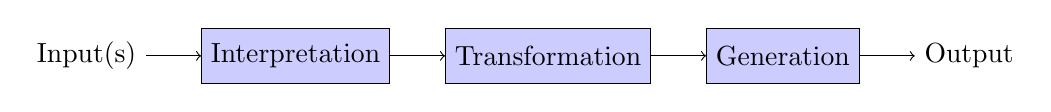
\begin{tikzpicture}[node distance=0.7cm, auto]
\node (input) [] {Input(s)};
\node (interpretation) [block, right =of input] {Interpretation};
\node (transformation) [block, right =of interpretation] {Transformation};
\node (generation) [block, right =of transformation] {Generation};
\node (output) [right =of generation] {Output};
\draw [->] (input) -- (interpretation);
\draw [->] (interpretation) -- (transformation);
\draw [->] (transformation) -- (generation);
\draw [->] (generation) -- (output);
\end{tikzpicture}
\caption{\cite{lloret_text_2008} Summarization Steps}
\label{fig:summarization_steps}
\end{figure}

- Do same as project (main core with acronym like SumASG, then SumASG* to fix/build on top of foundation)
    - Use Peter Little examples
    - Appendix with summary generation rules
    - Talk about expandability (talk about mechanisms)
    - Very nice to not be able to generate grammatically incorrect with ASG
- Describe action predicates as high level semantic descriptor of all possible actions that can happen in sentences
- Think about initial motivation (have definition of what is summary, NN does not)
    1. NNs need lots of data and time to summarize
    2. ASG can give results with short list of rules, pre/post-processing and carefully constructed structure
- Maybe formalize mathematically task of summarization (with CFG, BK, E+, E-)
    1. CFG is language, BK is leaf nodes, result is actions
    2. CFG is language, BK is leaf nodes, E is actions, result is summaries
- For report think about how to formalize task of summarization in ASG (how thought evolve)
    1. Originally just create summaries from actions
    2. Now preprocess to prune and homogenize, produce and score summaries, take best and fix grammar
    3. Use example of Peter Little to showcase pipeline
- Compare with NN
    1. Randomize action(...) to generate summary(...) on trained ASG
    2. Train NN to generate same summary(...)
    3. Show framework is sane and expandable (computationally tractable)
    4. Compute Rouge score (PyRouge, must clone repo into project) on ASG and NN
- Final goal: take story-specific ASG and general rules to generate summaries, then use top 5/10

\chapter{Preprocessor}
\label{chapter:preprocessor}

\section{Overview}

In order to prepare the story to be parsed and summarized by \textsc{SumASG}, we have created the \textsc{Preprocessor}. As we will loose information in summary anyway, it is completely acceptable to... which steps are shown below in Figure \ref{fig:preprocessor_pipeline}.

\begin{figure}[H]
\centering
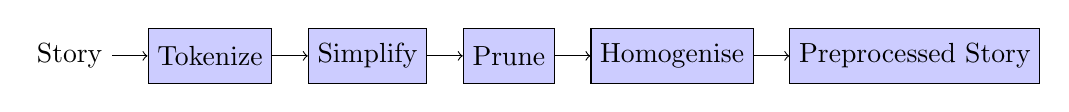
\begin{tikzpicture}[node distance=0.45cm, auto]
\node (story_in) [] {Story};
\node (tokenize) [block, right =of story_in] {Tokenize};
\node (simplify) [block, right =of tokenize] {Simplify};
\node (prune) [block, right =of simplify] {Prune};
\node (homogenise) [block, right =of prune] {Homogenise};
\node (story_out) [block, right =of homogenise] {Preprocessed Story};
\draw [->] (story_in) -- (tokenize);
\draw [->] (tokenize) -- (simplify);
\draw [->] (simplify) -- (prune);
\draw [->] (prune) -- (homogenise);
\draw [->] (homogenise) -- (story_out);
\end{tikzpicture}
\caption{Preprocessor Steps}
\label{fig:preprocessor_pipeline}
\end{figure}

\section{Tokenization And Simplification}
\label{sec:tokenization_scoring}

With the help of \textbf{CoreNLP}, we can assign a POS tag to each word, or \textit{token}, from the input story. Using this information, we can now make a number of simplifications which will make the sentence structure more consistent throughout.

\subsection{Punctuation}
\label{subsec:punctuation}

To avoid having to build recognition and semantic understanding of different types of punctuation into \textsc{SumASG}, it is preferable to transform the story such that it uses no punctuation apart from full stops. The idea is that each sentence in the resulting text contains exactly one action or description.

Depending on the type of punctuation used at the end of a clause, a different treatment is applied:
\begin{itemize}[nolistsep]
\item Question marks: We remove the clause, as it is most likely irrelevant for this task. It also helps avoid negation since we are deleting rhetorical questions.
\item Dashes: These are used around clauses which add detail, so it is quite safe to delete them for the task of summarization.
\item Exclamation marks, commas, semi-colons and colons: We replace any of these with a full stop.
\end{itemize}

\subsection{Individual Word Transformations}

One of the main goals of the \textsc{Preprocessor} is to transform the story in a simple and consistent structure, one where a given POS tag may only appear in a limited number of places in a sentence.

\subsubsection{Acronyms}

Some acronyms are often spelled using full stops after each letter. To prevent these from being recognized as multiple sentences, it is beneficial to remove any punctuation from acronyms. Therefore the word ``U.S.A." would become ``USA".

\subsubsection{Contractions}

Contractions can be difficult to understand for machines, and they add unwanted complexity to the task of parsing. Therefore it is simplest to expand all of them, for example transforming ``it's" into ``it is".

\subsubsection{Adverbs}

In the English language, adverbs can appear almost anywhere in a sentence, and their position has minimal semantic influence. To illustrate this, consider the following sentences, which all have the same meaning:

\begin{displayquote}
\underline{Slowly} he eats toast. \\
He \underline{slowly} eats toast. \\
He eats toast \underline{slowly}.
\end{displayquote}

In order to provide \textsc{SumASG} with a consistent format for parsing adverbs, we should always move them to the end of the clause in which they appear (in the above example we would keep the last sentence).


\subsubsection{Determiners}

In the English language, the determiners ``a" and ``an" are semantically identical, so to makes sense to only use one of the two, with the intention of reducing the number of \textit{tokens} that \textsc{SumASG has to process}. We can always correct the output of \textsc{SumASG} to make it grammatically-correct.

\subsubsection{Possessive Pronouns, Interjections And Prepositions}

In most cases, possessive pronouns and interjections do not add much to the meaning of a story, especially when the end goal is to create a summary. Therefore, we can remove such words from the text. For instance, the sequence ``\underline{Ah}! She ate \underline{her} chocolate." would become ``She ate chocolate.".

Prepositions which appear at the start of a sentence may be removed, as they are not integral to the meaning. For example, ``\underline{Besides} today is Sunday" gets transformed into ``Today is Sunday".

Moreover, prepositions which come after the object in a sentence can sometimes cause it to become syntactically too complex. Rather than encoding such high-level of detail into the internal representation of \textsc{SumASG}, it is preferable to simply omit the final clause. In this case, ``They have a picnic \underline{under} a tree." becomes ``They have a picnic.". Although some information is thrown away, this loss will usually have no impact on the quality of the summary.

\subsection{Clause Transformations}

After going through the \textsc{Preprocessor}, we would like each sentence in the given story to only focus on a single topic.

When possible, we should split sentences containing multiple clauses into individual sentences. Otherwise, we can delete the auxiliary clause and keep the main clause.

Examples of the transformations applied to different types of clauses can be seen below in Figure \ref{fig:clause_transformations}.

\begin{figure}[H]
\begin{subfigure}{\textwidth}
\begin{displayquote}
\textit{Conjunctive Clause} We looked left \underline{and} they saw us.\\
\textit{Conjunctive Clause}. Cars have wheels \underline{and} go fast.\\
\textit{Subordinating Clause}. She never walks alone \underline{because} she is afraid.\\
\textit{Dependant Clause}. I want to be President \underline{when I grow up}.\\
\textit{Dependant Clause}. \underline{When I grow up}, I will have a garden.
\end{displayquote}
\caption{Before transformation}
\vspace{\baselineskip}
\end{subfigure}
\begin{subfigure}{\textwidth}
\begin{displayquote}
\textit{Conjunctive Clause}. We looked left. they saw us.\\
\textit{Conjunctive Clause}. Cars have wheels. Cars go fast.\\
\textit{Subordinating Clause}. She never walks alone. she is afraid.\\
\textit{Dependant Clause}. I want to be President.\\
\textit{Dependant Clause}. I will have a garden.
\caption{After transformation}
\end{displayquote}
\end{subfigure}
\caption{Examples of the splitting of multi-clause sentences}
\label{fig:clause_transformations}
\end{figure}

\subsubsection{Hypernym Substitution}

However, in some cases we may be able to perform an optimization that allows us to collapse a conjunction of two words into a common \textit{hypernym} (i.e. superclass).

In practice, this involves using \textbf{\href{http://web.archive.org/web/20190516161631/https://www.clips.uantwerpen.be/pages/pattern-en}{Pattern}} to try and find a lexical field to which both words pertain.

For example, the words ``chicken" and ``goose" both belong to the lexical field of ``poultry". Similarly, ``cars" and ``trucks" have common hypernym ``motor-vehicles".

\textcolor{red}{\textbf{\hl{TODO give more details about how chosen?}}}

\subsection{Case And Proper Nouns}

We want to ensure that all occurrences of a word are treated as the same \textit{token}. Since \textsc{SumASG} will be generating new sentences from scratch, the simplest solution is to convert the entire story to lower-case, apart from proper nouns.

In the case of complex proper nouns (i.e., those constructed from multiple words), we should remove inner spaces so that we end up with a camel-case string. For instance, the sequence ``Peter Little" will become ``PeterLittle".

We can also do this with complex common nouns, for example transforming ``bird house" into ``bird-house".

\subsubsection{Pronoun Substitution}

Sometimes, an author will introduce a character or group by name, and later refer to them using a pronoun.

If a story contains exactly one distinct singular proper noun and then uses either ``he" or ``she", then it is safe to assume that this pronoun refers the aforementioned proper noun. The same can be said about plural proper nouns and the pronoun ``they".
To clarify this, an example is shown in Figure \ref{fig:pronoun_substitution}.

\begin{figure}[H]
\begin{subfigure}{\textwidth}
\begin{displayquote}
\textbf{Antonio} is a cheesemaker. \underline{He} makes burrata.
\textbf{Italians} eat pasta. \underline{They} make it with egg sometimes.
\end{displayquote}
\caption{Before transformation}
\vspace{\baselineskip}
\end{subfigure}
\begin{subfigure}{\textwidth}
\begin{displayquote}
\textbf{Antonio} is a cheesemaker. \textbf{Antonio} makes burrata.
\textbf{Italians} eat pasta. \textbf{Italians} make it with egg sometimes.
\caption{After transformation}
\end{displayquote}
\end{subfigure}
\caption{Example of substituting pronouns with proper nouns}
\label{fig:pronoun_substitution}
\end{figure}

\subsection{Example}
\label{subsec:simplification_example}

The result of running the simplification transformations is illustrated below in Figure \ref{fig:simplification_example}. Please refer to Chapter \ref{chapter:contributions} for the original story.

\begin{figure}[H]
\begin{subfigure}{\textwidth}
\begin{displayquote}
\begin{enumerate}[label=\protect\circled{\alph*}]
\item Adverbs: move ``always" and ``Now" to the end of the sentence
\item Determiners: ``an" $\rightarrow$ ``a"
\item Possessive pronouns: \st{``his"}
\item Prepositions: \st{``So"}
\item Conjunctive clauses: ``serious in school" $\|$ ``did homework always"
\item Dependant clauses: \st{``When he was older"}
\item Complex clauses: ``was a curious little boy" $\|$ ``named Peter Little"
\item Hypernym substitution: ``stars and planets" $\rightarrow$ ``astronomy"
\item Case: make all words but proper nouns lower case
\item Complex nouns: ``Peter Little" $\rightarrow$ ``PeterLittle"
\item Complex nouns: ``quantum physics" $\rightarrow$ ``quantum-physics"
\item Pronoun substitution: ``he" $\rightarrow$ ``PeterLittle"
\end{enumerate}
\end{displayquote}
\caption{Transformations applied (where $\|$ means splitting into multiple sentences)}
\vspace{\baselineskip}
\end{subfigure}
\begin{subfigure}{\textwidth}
\begin{displayquote}
\textbf{0.} there was a curious little boy.\\
\textbf{1.} \circled{g} the curious little boy was named \circled{j} PeterLittle.\\
\textbf{2.} \circled{l} PeterLittle was interested in \circled{h} astronomy.\\
\textbf{3.} \circled{d} PeterLittle was serious in school.\\
\textbf{4.} \circled{e} PeterLittle did \circled{c} homework \circled{a} always.\\
\textbf{5.} \circled{f} PeterLittle studied mathematics and \circled{k} quantum-physics.\\
\textbf{6.} PeterLittle studied for \circled{c} exams hard.\\
\textbf{7.} PeterLittle became \circled{b} a astrophysicist.\\
\textbf{8.} PeterLittle is famous \circled{a} now.
\caption{Sentences after applying transformations}
\end{displayquote}
\end{subfigure}
\caption{Example of applying \textit{simplification} to the story of Peter Little}
\label{fig:simplification_example}
\end{figure}

\section{Sentence Pruning And Homogenization}

Once the sentence structure of the story has been \textit{simplified}, one of the main jobs of the \textsc{Preprocessor} is to remove irrelevant semantic complexity from the story.

In order to understand what is relevant in a story and what is not, the \textsc{Preprocessor} looks at the semantic similarity between words with the same POS tag (or a related one, i.e. singular noun and plural noun, or verbs with a different tense).

\subsection{Word Similarity}

It uses a loop to iterate over each sentence, and compares each word with every word from other sentences which have the same or a related POS tag. For each comparison, word \textit{similarity} is computed using the tool \href{http://www.conceptnet.io}{ConceptNet}, a semantic knowledge network.

As you might imagine, having such nesting of loops can be quite expensive, which is why we keep a cache of previously requested similarities, and use the fact that this \textit{similarity} relation is symmetric.

\subsection{Sentence Similarity And Pruning}

\subsubsection{Sentence Similarity}

Once we have computed the \textit{similarity} between words of different sentences, we can add these up on a per-sentence basis, which gives us a binary relation of \textit{similarity} between sentences.

We now have enough information to generate a \textit{text relationship map} over the sentences. The idea is that the more ``linked" a sentence is, the more relevant it is to the story. For each sentence, we therefore take the sum of the values of all its \textit{similarity} relations with other sentences. The higher this number, the more relevant, or \textit{important}, the sentence is to the story.

\subsubsection{Pruning}

In the interest of removing irrelevant sentences to help \textsc{SumASG}, we compute the 25th percentile over the \textit{importances} of all the sentences. We then prune sentences whose \textit{importance} is strictly less than this value.

In most cases, one quarter of the story will be pruned. However, if every sentence has the same \textit{importance}, then nothing gets removed. On the other hand, if two thirds of the story are very \textit{important} and the rest is irrelevant, then we remove more than a quarter of the sentences.

\subsection{Synonyms And Homogenization}

Another use for \textit{word similarity} is to find out if the author of the story has used any synonyms. When the \textit{similarity} between two words is above a certain threshold, then we consider them to be synonyms.

For every set of synonyms we find, we can choose a unique \textit{representative} for the set, and replace occurrences of the other words in that set with our \textit{representative}. For simplicity, we choose the \textit{representative} as the shortest word in its synonym set.

This is what we call \textit{story homogenization}, and it helps \textsc{SumASG} link words that would otherwise be considered completely different \textit{tokens} in the story.

\subsection{Example}

An example is shown below in Figure \ref{fig:preprocessor_example} for the story of Peter Little, where the weight between two nodes denotes \textit{similarity}. In this example, we consider words to be synonyms whenever their \textit{similarity} is at least 20. The labels of the nodes (starting from 0) for sentence \textit{similarity} correspond to the index of the sentence in the \textit{simplified story} (see Subsection \ref{subsec:simplification_example}).

As you can see, sentences 5 and 6 are deemed irrelevant and will be pruned, while sentences 0, 1 and 2 are thought as being very important.

Moreover, {homework, school} and {interested, curious} are considered synonym sets, and \textit{homogenization} will replace occurrences of these words with their shortest synonym (which may be itself).

\begin{figure}[H]
\begin{subfigure}{\textwidth}
\begin{subfigure}{0.5\textwidth}
\renewcommand\thesubfigure{\roman{subfigure}}
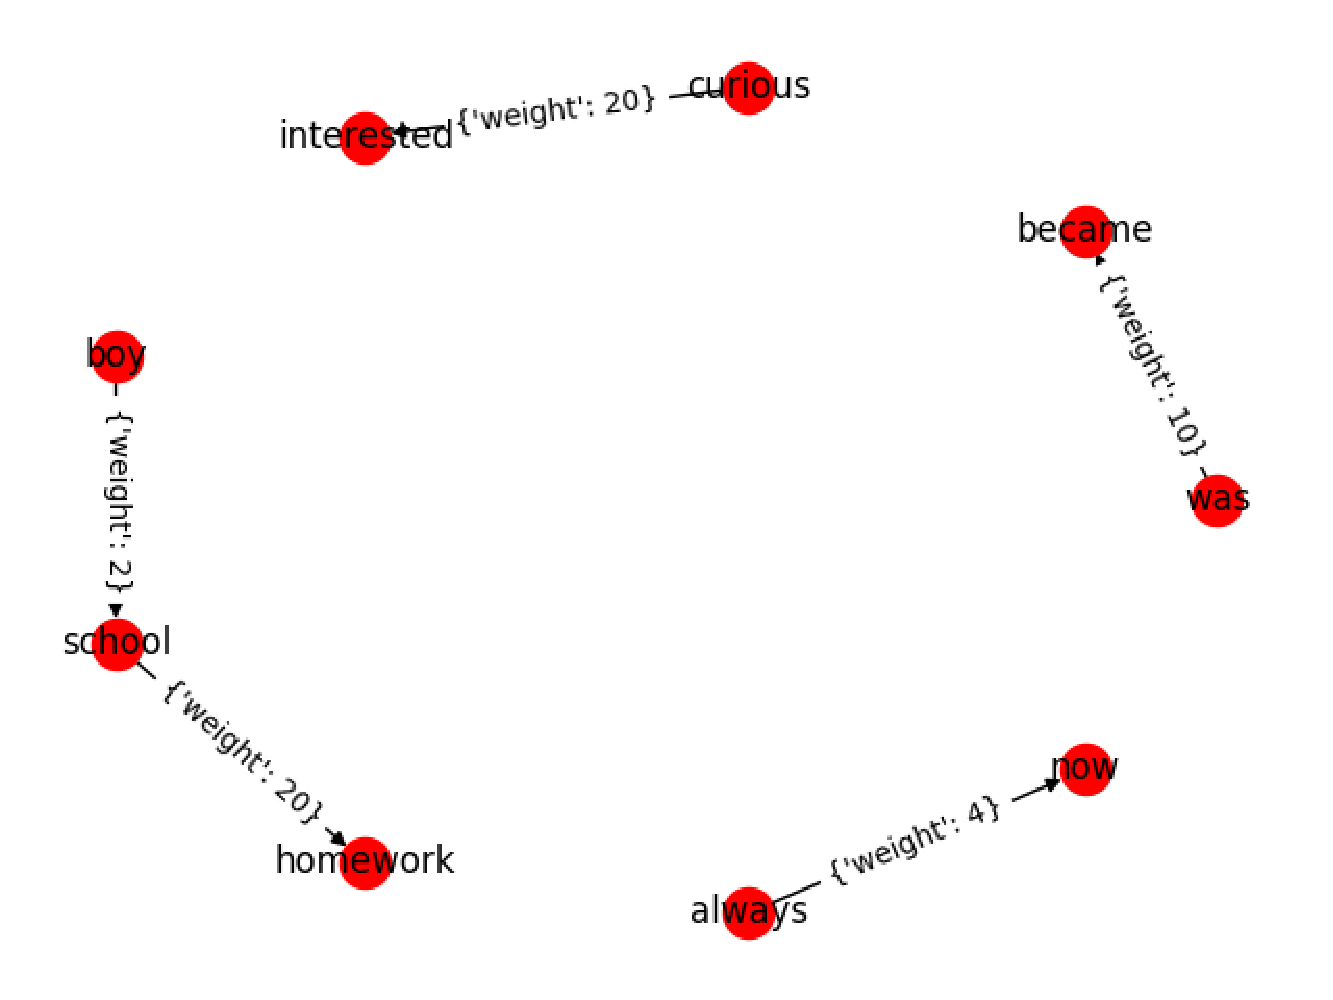
\includegraphics[width=\textwidth]{word_similarity.eps}
\caption{Word \textit{similarity}}
\end{subfigure}
\begin{subfigure}{0.5\textwidth}
\renewcommand\thesubfigure{\roman{subfigure}}
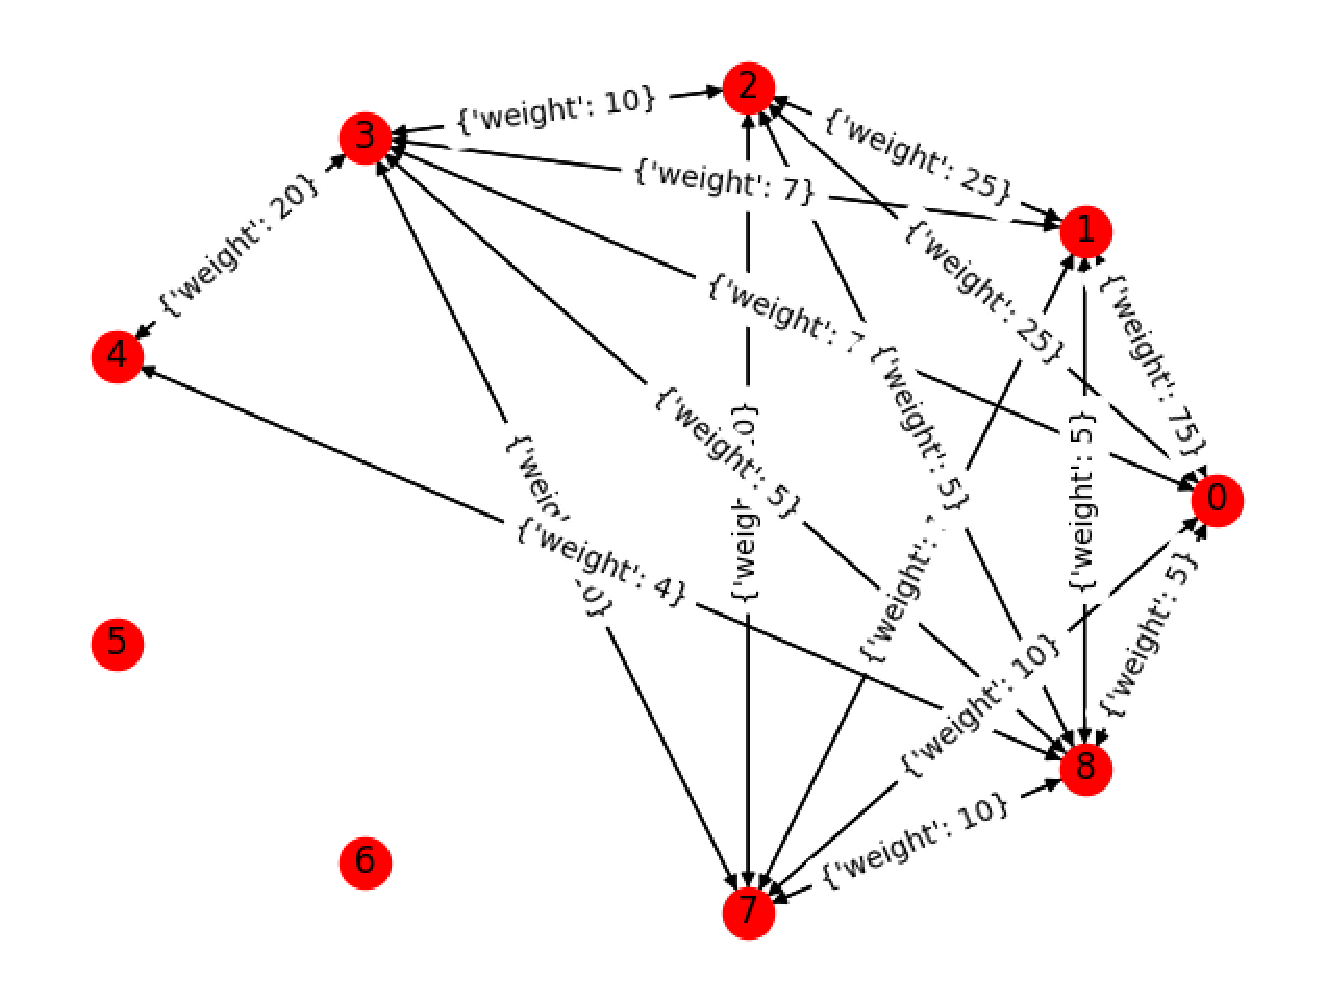
\includegraphics[width=\textwidth]{sentence_similarity.eps}
\caption{Sentence \textit{similarity}}
\end{subfigure}
\setcounter{subfigure}{0}
\caption{\textit{Text relationship maps}}
\end{subfigure}
\begin{subfigure}{\textwidth}
\vspace{\baselineskip}
\centering
\begin{tabular}{@{}llllllllll@{}}
\toprule
Sentence   & 0    & 1    & 2    & 3    & 7    & 8    & 4 & 5 & 6 \\ \midrule
Importance & 40.7 & 24.4 & 18.8 & 14.8 & 12.5 & 11.3 & 6 & 0 & 0 \\ \bottomrule
\end{tabular}
\caption{Sentences ordered by importance}
\end{subfigure}
\begin{subfigure}{\textwidth}
\vspace{\baselineskip}
\begin{displayquote}
there was a curious little boy. the curious little boy was named PeterLittle. PeterLittle was curious in astronomy. PeterLittle was serious in school. PeterLittle did school always. PeterLittle became a astrophysicist. PeterLittle is famous now.
\end{displayquote}
\caption{\textit{Homogenized} story}
\end{subfigure}
\caption{Example of applying sentence pruning and \textit{homogenization} to the \textit{simplified} story of Peter Little}
\label{fig:preprocessor_example}
\end{figure}

\section{Expandability}

In its current state, \textsc{SumASG} expects positive sentences only, and the only form of punctuation recognized is the full stop.

\subsection{Negation}

In order to support negation, we would need to modify the structure of \textsc{SumASG}'s internal representation (see Chapter \ref{chapter:asg}). However, to achieve a better semantic understanding in \textsc{SumASG*}, we could add some more simplification logic to the \textsc{Preprocessor}.

After having implemented this, the phrase ``not happy" would be transformed into the word ``sad".

\subsection{Lists}

At the moment, \textsc{SumASG} can parse a list of length 2 at the most, i.e. a conjunction of two items. By adding a transformation to the \textsc{Preprocessor} before we modify the punctuation (see Subsection \ref{subsec:punctuation}), we could overcome this limitation. Intuitively, this would mean going from a sentence with a an $n$-item list, to $\floor{\frac{n}{2}}$ sentences with two objects and one sentence with a single object (if $n$ is odd).

For instance, the sentence ``Bob had a book, a computer and a chair." would be split into ``Bob had a book and a computer. Bob had a chair".

Choice:
1. Simplify using Python script (faster)
2. Make ASG format more complex (new information probably lost in summary anyway)

- Punctuation
    - [?]: remove clause (helps avoid negation for rhetorical questions)
    - [!|,|;|:]: transform into '.'
    - [–|—]: delete inner part
- Multiple clauses (conjunctive or main+auxiliary): split into multiple sentences
- Adverbs: move to end
- Possessive pronouns and interjections: remove
- Prepositions: remove when at start of sentence
- Contractions: expand
- Acronyms: remove punctuation
- Dependant clauses: split into separate sentence (remove if there is no punctuation)
- Verbless sentences: remove
- Subordinating conjunctions: split into separate sentence
- Preposition clauses: remove if after object
- Complex proper nouns: collapse into CamelCase
- Proper nouns: replace occurrences of pronouns with relevant proper noun (idea: if they are used in the story then there should be little ambiguity)
- Conjunction of common nouns from same lexical field: replace with hypernym (pluralize if items are plural and hypernym plural is used in English)

\chapter{ASG}
\chapter{ASG}

\textcolor{red}{\textbf{\hl{TODO fix margin, separate task1 from task2 code}}}

\begin{lstlisting}
start -> s_group {
   :- count(X)@1, X > 1.
   :- count(X)@1, X = 0.
}

s_group -> {
  count(0).
}

s_group -> s_group s ". " {
  count(X+1) :- count(X)@1.

  % Reject output summaries with duplicate sentences
  sentence(X,V,O,S) :- output(_,V,O,S)@2, count(X).
  sentence(X,V,O,S) :- sentence(X,V,O,S)@1.
  :- sentence(X1,V,O,S), sentence(X2,V,O,S), X1 != X2.
}

s -> np vp {
  :- not action(verb(V_N,V_T),subject(S_N,S_D,S_A),object(O_N,O_D,O_A)), verb(V_N,V_T)@2, subject(S_N,S_D,S_A)@1, object(O_N,O_D,O_A)@2.

  subject :- subject(S_N,S_D,S_A)@1.
  :- not subject.
  object :- object(S_N,S_D,S_A)@2.
  :- not object.
}

vp -> vbn np {
  verb(N,T) :- verb(N,T)@1.
  object(N,D,A) :- object(N,D,A)@2.
}

vp -> vbd np {
  verb(N,T) :- verb(N,T)@1.
  object(N,D,A) :- object(N,D,A)@2.
}

vp -> vbd vbg np {
  verb(comp(N1,N2),comp(T1,gerund)) :- verb(N1,T1)@1, verb(N2,gerund)@2.
  object(N,D,A) :- object(N,D,A)@3.
}

vp -> vbd vbn np {
  verb(comp(N1,N2),comp(T1,past_part)) :- verb(N1,T1)@1, verb(N2,past_part)@2.
  object(N,D,A) :- object(N,D,A)@3.
}

vp -> vbd "to " vb np {
  verb(comp(N1,N2),comp(T1,base)) :- verb(N1,T1)@1, verb(N2,base)@3.
  object(N,D,A) :- object(N,D,A)@4.
}

vp -> vbp np {
  verb(N,T) :- verb(N,T)@1.
  object(N,D,A) :- object(N,D,A)@2.
}

vp -> vbp vbg np {
  verb(comp(N1,N2),comp(T1,gerund)) :- verb(N1,T1)@1, verb(N2,gerund)@2.
  object(N,D,A) :- object(N,D,A)@3.
}

vp -> vbp vbn np {
  verb(comp(N1,N2),comp(T1,past_part)) :- verb(N1,T1)@1, verb(N2,past_part)@2.
  object(N,D,A) :- object(N,D,A)@3.
}

vp -> vbp "to " vb np {
  verb(comp(N1,N2),comp(T1,base)) :- verb(N1,T1)@1, verb(N2,base)@3.
  object(N,D,A) :- object(N,D,A)@4.
}

vp -> vbz np {
  verb(N,T) :- verb(N,T)@1.
  object(N,D,A) :- object(N,D,A)@2.
}

vp -> vbz vbg np {
  verb(comp(N1,N2),comp(T1,gerund)) :- verb(N1,T1)@1, verb(N2,gerund)@2.
  object(N,D,A) :- object(N,D,A)@3.
}

vp -> vbz vbn np {
  verb(comp(N1,N2),comp(T1,past_part)) :- verb(N1,T1)@1, verb(N2,past_part)@2.
  object(N,D,A) :- object(N,D,A)@3.
}

vp -> vbz "to " vb np {
  verb(comp(N1,N2),comp(T1,base)) :- verb(N1,T1)@1, verb(N2,base)@3.
  object(N,D,A) :- object(N,D,A)@4.
}

np -> np rb {
  object(N,D,A) :- object(N,D,0)@1, adj_or_adv(A)@2.
}

np -> np rb {
  object(N,D,conjunct(A1,A2)) :- object(N,D,A1)@1, adj_or_adv(A2)@2.
  :- object(N,D,conjunct(A,A)).
}

np -> np rp {
  object(N,D,A) :- object(N,D,0)@1, adj_or_adv(A)@2.
}

np -> np rp {
  object(N,D,conjunct(A1,A2)) :- object(N,D,A1)@1, adj_or_adv(A2)@2.
  :- object(N,D,conjunct(A,A)).
}

np -> nn {
  subject(N,0,0) :- noun(N)@1.
  object(N,0,0) :- noun(N)@1.
}

np -> nns {
  subject(N,0,0) :- noun(N)@1.
  object(N,0,0) :- noun(N)@1.
}

np -> nnp {
  subject(N,0,0) :- noun(N)@1.
  object(N,0,0) :- noun(N)@1.
}

np -> nnps {
  subject(N,0,0) :- noun(N)@1.
  object(N,0,0) :- noun(N)@1.
}

np -> prp {
  subject(N,0,0) :- noun(N)@1.
  object(N,0,0) :- noun(N)@1.
}

np -> rb {
  subject(0,0,A) :- adj_or_adv(A)@1.
  object(0,0,A) :- adj_or_adv(A)@1.
}

np -> rp {
  subject(0,0,A) :- adj_or_adv(A)@1.
  object(0,0,A) :- adj_or_adv(A)@1.
}

np -> ex {
  subject(N,0,0) :- noun(N)@1.
}

np -> in {
  object(0,D,0) :- det(D)@1.
}

np -> prp "and " nnp {
  subject(conjunct(N1,N2),0,0) :- noun(N1)@1, noun(N2)@3.
  object(conjunct(N1,N2),0,0) :- noun(N1)@1, noun(N2)@3.
  :- subject(conjunct(N,N),0,0).
  :- object(conjunct(N,N),0,0).
}

np -> nnp "and " prp {
  subject(conjunct(N1,N2),0,0) :- noun(N1)@1, noun(N2)@3.
  object(conjunct(N1,N2),0,0) :- noun(N1)@1, noun(N2)@3.
  :- subject(conjunct(N,N),0,0).
  :- object(conjunct(N,N),0,0).
}

np -> dt nn "and " prp {
  subject(conjunct(N1,N2),D,0) :- det(D)@1, noun(N1)@2, noun(N2)@4.
  object(conjunct(N1,N2),D,0) :- det(D)@1, noun(N1)@2, noun(N2)@4.
  :- subject(conjunct(N,N),_,0).
  :- object(conjunct(N,N),_,0).
}

np -> prp "and " dt nn {
  subject(conjunct(N1,N2),D,0) :- noun(N1)@1, det(D)@3, noun(N2)@4.
  object(conjunct(N1,N2),D,0) :- noun(N1)@1, det(D)@3, noun(N2)@4.
  :- subject(conjunct(N,N),_,0).
  :- object(conjunct(N,N),_,0).
}

np -> dt nn "and " nnp {
  subject(conjunct(N1,N2),D,0) :- det(D)@1, noun(N1)@2, noun(N2)@4.
  object(conjunct(N1,N2),D,0) :- det(D)@1, noun(N1)@2, noun(N2)@4.
  :- subject(conjunct(N,N),_,0).
  :- object(conjunct(N,N),_,0).
}

np -> nnp "and " dt nn {
  subject(conjunct(N1,N2),D,0) :- noun(N1)@1, det(D)@3, noun(N2)@4.
  object(conjunct(N1,N2),D,0) :- noun(N1)@1, det(D)@3, noun(N2)@4.
  :- subject(conjunct(N,N),_,0).
  :- object(conjunct(N,N),_,0).
}

np -> nnp "and " nnp {
  subject(conjunct(N1,N2),0,0) :- noun(N1)@1, noun(N2)@3.
  object(conjunct(N1,N2),0,0) :- noun(N1)@1, noun(N2)@3.
  :- subject(conjunct(N,N),0,0).
  :- object(conjunct(N,N),0,0).
}

np -> nn "and " nn {
  subject(conjunct(N1,N2),0,0) :- noun(N1)@1, noun(N2)@3.
  object(conjunct(N1,N2),0,0) :- noun(N1)@1, noun(N2)@3.
  :- subject(conjunct(N,N),0,0).
  :- object(conjunct(N,N),0,0).
}

np -> nn "and " nns {
  subject(conjunct(N1,N2),0,0) :- noun(N1)@1, noun(N2)@3.
  object(conjunct(N1,N2),0,0) :- noun(N1)@1, noun(N2)@3.
  :- subject(conjunct(N,N),0,0).
  :- object(conjunct(N,N),0,0).
}

np -> nns "and " nn {
  subject(conjunct(N1,N2),0,0) :- noun(N1)@1, noun(N2)@3.
  object(conjunct(N1,N2),0,0) :- noun(N1)@1, noun(N2)@3.
  :- subject(conjunct(N,N),0,0).
  :- object(conjunct(N,N),0,0).
}

np -> nns "and " nns {
  subject(conjunct(N1,N2),0,0) :- noun(N1)@1, noun(N2)@3.
  object(conjunct(N1,N2),0,0) :- noun(N1)@1, noun(N2)@3.
  :- subject(conjunct(N,N),0,0).
  :- object(conjunct(N,N),0,0).
}

np -> prp "and " prp {
  subject(conjunct(N1,N2),0,0) :- noun(N1)@1, noun(N2)@3.
  object(conjunct(N1,N2),0,0) :- noun(N1)@1, noun(N2)@3.
  :- subject(conjunct(N,N),0,0).
  :- object(conjunct(N,N),0,0).
}

np -> rb "and " rb {
  subject(0,0,conjunct(A1,A2)) :- adj_or_adv(A1)@1, adj_or_adv(A2)@3.
  object(0,0,conjunct(A1,A2)) :- adj_or_adv(A1)@1, adj_or_adv(A2)@3.
  :- subject(0,0,conjunct(A,A)).
  :- object(0,0,conjunct(A,A)).
}

np -> jj {
  object(0,0,A) :- adj_or_adv(A)@1.
}

np -> jj "and " jj {
  object(0,0,conjunct(A1,A2)) :- adj_or_adv(A1)@1, adj_or_adv(A2)@3.
  :- object(0,0,conjunct(A,A)).
}

np -> jj rb {
  subject(0,0,conjunct(A1,A2)) :- adj_or_adv(A1)@1, adj_or_adv(A2)@1.
  object(0,0,conjunct(A1,A2)) :- adj_or_adv(A1)@1, adj_or_adv(A2)@1.
  :- subject(0,0,conjunct(A,A)).
  :- object(0,0,conjunct(A,A)).
}

np -> dt nn {
  subject(N,D,0) :- det(D)@1, noun(N)@2.
  object(N,D,0) :- det(D)@1, noun(N)@2.
}

np -> dt nns {
  subject(N,D,0) :- det(D)@1, noun(N)@2.
  object(N,D,0) :- det(D)@1, noun(N)@2.
}

np -> jj nns {
  subject(N,0,A) :- adj_or_adv(A)@1, noun(N)@2.
  object(N,0,A) :- adj_or_adv(A)@1, noun(N)@2.
}

np -> jj nnp {
  subject(N,0,A) :- adj_or_adv(A)@1, noun(N)@2.
  object(N,0,A) :- adj_or_adv(A)@1, noun(N)@2.
}

np -> jj nnps {
  subject(N,0,A) :- adj_or_adv(A)@1, noun(N)@2.
  object(N,0,A) :- adj_or_adv(A)@1, noun(N)@2.
}

np -> dt jj nn {
  subject(N,D,A) :- det(D)@1, adj_or_adv(A)@2, noun(N)@3.
  object(N,D,A) :- det(D)@1, adj_or_adv(A)@2, noun(N)@3.
}

np -> dt jj nns {
  subject(N,D,A) :- det(D)@1, adj_or_adv(A)@2, noun(N)@3.
  object(N,D,A) :- det(D)@1, adj_or_adv(A)@2, noun(N)@3.
}

np -> dt jj jj nn {
  subject(N,D,conjunct(A1,A2)) :- det(D)@1, adj_or_adv(A1)@2, adj_or_adv(A2)@3, noun(N)@4.
  object(N,D,conjunct(A1,A2)) :- det(D)@1, adj_or_adv(A1)@2, adj_or_adv(A2)@3, noun(N)@4.
  :- subject(N,D,conjunct(A,A)).
  :- object(N,D,conjunct(A,A)).
}

np -> dt jj jj nns {
  subject(N,D,conjunct(A1,A2)) :- det(D)@1, adj_or_adv(A1)@2, adj_or_adv(A2)@3, noun(N)@4.
  object(N,D,conjunct(A1,A2)) :- det(D)@1, adj_or_adv(A1)@2, adj_or_adv(A2)@3, noun(N)@4.
  :- subject(N,D,conjunct(A,A)).
  :- object(N,D,conjunct(A,A)).
}

np -> dt jjr nn {
  subject(N,D,A) :- det(D)@1, adj_or_adv(A)@2, noun(N)@3.
  object(N,D,A) :- det(D)@1, adj_or_adv(A)@2, noun(N)@3.
}

np -> dt jjr nns {
  subject(N,D,A) :- det(D)@1, adj_or_adv(A)@2, noun(N)@3.
  object(N,D,A) :- det(D)@1, adj_or_adv(A)@2, noun(N)@3.
}

np -> dt jjs nn {
  subject(N,D,A) :- det(D)@1, adj_or_adv(A)@2, noun(N)@3.
  object(N,D,A) :- det(D)@1, adj_or_adv(A)@2, noun(N)@3.
}

np -> dt jjs nns {
  subject(N,D,A) :- det(D)@1, adj_or_adv(A)@2, noun(N)@3.
  object(N,D,A) :- det(D)@1, adj_or_adv(A)@2, noun(N)@3.
}

np -> in nn {
  object(N,D,0) :- det(D)@1, noun(N)@2.
}

np -> in dt nn {
  object(N,conjunct(D1,D2),0) :- det(D1)@1, det(D2)@2, noun(N)@3.
}

np -> in nns {
  object(N,D,0) :- det(D)@1, noun(N)@2.
}

np -> in dt nns {
  object(N,conjunct(D1,D2),0) :- det(D1)@1, det(D2)@2, noun(N)@3.
}

np -> in nnp {
  object(N,D,0) :- det(D)@1, noun(N)@2.
}

np -> in nnps {
  object(N,D,0) :- det(D)@1, noun(N)@2.
}

np -> jj in nn {
  object(N,D,A) :- adj_or_adv(A)@1, det(D)@2, noun(N)@3.
}

np -> jj in nn "and " nn {
  object(conjunct(N1,N2),D,A) :- adj_or_adv(A)@1, det(D)@2, noun(N1)@3, noun(N2)@5.
}

np -> jj in nns {
  object(N,D,A) :- adj_or_adv(A)@1, det(D)@2, noun(N)@3.
}

np -> jj in nns "and " nns {
  object(conjunct(N1,N2),D,A) :- adj_or_adv(A)@1, det(D)@2, noun(N1)@3, noun(N2)@5.
}

np -> jj in nnp {
  object(N,D,A) :- adj_or_adv(A)@1, det(D)@2, noun(N)@3.
}

np -> jj in nnp "and " nnp {
  object(conjunct(N1,N2),D,A) :- adj_or_adv(A)@1, det(D)@2, noun(N1)@3, noun(N2)@5.
}

np -> jj in prp {
  object(N,D,A) :- adj_or_adv(A)@1, det(D)@2, noun(N)@3.
}

np -> jj in prp "and " prp {
  object(conjunct(N1,N2),D,A) :- adj_or_adv(A)@1, det(D)@2, noun(N1)@3, noun(N2)@5.
}

np -> jj in nn "and " nns {
  object(conjunct(N1,N2),D,A) :- adj_or_adv(A)@1, det(D)@2, noun(N1)@3, noun(N2)@5.
}

np -> jj in nns "and " nn {
  object(conjunct(N1,N2),D,A) :- adj_or_adv(A)@1, det(D)@2, noun(N1)@3, noun(N2)@5.
}

np -> cd nn {
  subject(N,D,0) :- det(D)@1, noun(N)@2.
  object(N,D,0) :- det(D)@1, noun(N)@2.
}

np -> cd nns {
  subject(N,D,0) :- det(D)@1, noun(N)@2.
  object(N,D,0) :- det(D)@1, noun(N)@2.
}

np -> cd jj nn {
  subject(N,D,A) :- det(D)@1, adj_or_adv(A)@2, noun(N)@3.
  object(N,D,A) :- det(D)@1, adj_or_adv(A)@2, noun(N)@3.
}

np -> cd jj nns {
  subject(N,D,A) :- det(D)@1, adj_or_adv(A)@2, noun(N)@3.
  object(N,D,A) :- det(D)@1, adj_or_adv(A)@2, noun(N)@3.
}

np -> cd nns jj {
  object(N,D,A) :- det(D)@1, noun(N)@2, adj_or_adv(A)@3.
}

np -> dt jj cd {
  subject(0,conjunct(D1,D2),A) :- det(D1)@1, adj_or_adv(A)@2, det(D2)@3.
  object(0,conjunct(D1,D2),A) :- det(D1)@1, adj_or_adv(A)@2, det(D2)@3.
}


\end{lstlisting}

- Learning is not really learning (ASG never learns how to summarize, we build in rules of feature extraction)

http://universalteacher.org.uk/lang/engstruct.htm

Ideas:
- final fix-up using language\_checker.fix
- hard-code determiners into derivations (https://www.ef.com/wwen/english-resources/english-grammar/determiners/)
- use lots of simple/precise rules rather than complicated/general ones to minimize ss
- keep rules as restricted as possible, when concept implemented over time add missing rules
- to avoid having to add grammar constraints try and rely on grammar of input

- reduce search space using mode bias (simple example: 396->16, very complicated example: 9477->1044)
- for learning actions do one sentence at a time to minimize ss
- pick best summary according to TTR*

action(INDEX, VERB, SUBJECT, OBJECT)
summary(VERB, SUBJECT, OBJECT)

verb(INDICATIVE\_FORM, TENSE)
subject(NOUN, DET, ADJ\_OR\_ADV)
object(NOUN, DET, ADJ\_OR\_ADV)
noun(NAME)
adj\_or\_adv(NAME)
det(...)
compound(FIRST, SECOND)  for verbs
conjunct(FIRST, SECOND)  learn both

* Type-Token Ratio (TTR): The basic idea behind that measure is that if the text is more complex, the author uses a more varied vocabulary so there’s a larger number of types (unique words). This logic is explicit in the TTR’s formula, which calculates the number of types divided by the number of tokens. As a result, the higher the TTR, the higher the lexical complexity.

\chapter{Post-Processing / Scoring}
\section{Overview}

Once we have obtained potential sentences from ASG to be used in a summary, we can now post-process these as explained in Section \ref{sec:summary_creation}. By combining them in different ways, we are able to form summaries. From these, we will retain the highest scoring ones, according to the metric detailed in Section \ref{sec:scoring}. A diagram illustrating these steps is shown below in Figure \ref{fig:postprocess_pipeline}.

\begin{figure}[H]
\centering
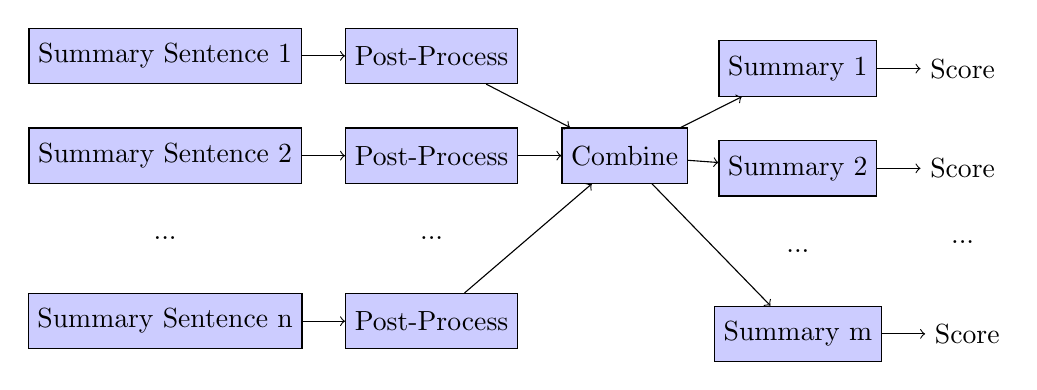
\begin{tikzpicture}[node distance=0.55cm, auto]
\node (summary_sentence_1) [block] {Summary Sentence 1};
\node (summary_sentence_2) [block, below =of summary_sentence_1] {Summary Sentence 2};
\node (summary_sentence_3) [below =of summary_sentence_2] {...};
\node (summary_sentence_4) [block, below =of summary_sentence_3] {Summary Sentence n};
\node (post_process_1) [block, right =of summary_sentence_1] {Post-Process};
\node (post_process_2) [block, below =of post_process_1] {Post-Process};
\node (post_process_3) [below =of post_process_2] {...};
\node (post_process_4) [block, below =of post_process_3] {Post-Process};
\node (combine) [block, right =of post_process_2] {Combine};
\node (summary_1) [block, above right =of combine] {Summary 1};
\node (summary_2) [block, below =of summary_1] {Summary 2};
\node (summary_3) [below =of summary_2] {...};
\node (summary_4) [block, below =of summary_3] {Summary m};
\node (score_1) [right =of summary_1] {Score};
\node (score_2) [below =of score_1, right =of summary_2] {Score};
\node (score_3) [below =of score_2] {...};
\node (score_4) [below =of score_3, right =of summary_4] {Score};
\draw [->] (summary_sentence_1) -- (post_process_1);
\draw [->] (summary_sentence_2) -- (post_process_2);
\draw [->] (summary_sentence_4) -- (post_process_4);
\draw [->] (post_process_1) -- (combine);
\draw [->] (post_process_2) -- (combine);
\draw [->] (post_process_4) -- (combine);
\draw [->] (combine) -- (summary_1);
\draw [->] (combine) -- (summary_2);
\draw [->] (combine) -- (summary_4);
\draw [->] (summary_1) -- (score_1);
\draw [->] (summary_2) -- (score_2);
\draw [->] (summary_4) -- (score_4);
\end{tikzpicture}
\caption{Post-Processing / Scoring Steps}
\label{fig:postprocess_pipeline}
\end{figure}

\section{Summary Creation}
\label{sec:summary_creation}

The output of \textsc{SumASG} is a list of sentences, each of which could potentially appear in the final summary.

\subsection{Post-Processing}

\subsubsection{Grammar}

Because \textsc{SumASG} uses the same capitalization for a given word regardless of its position in the sentence, it means that the first word of each sentence will not be capitalized unless it is a proper noun. We therefore need to fix this, as well as remove the space before each full stop.

Compound nouns, whose hyphen was replaced with an underscore for the internal representation of \textsc{SumASG}, also need to be restored to their grammatically-correct form.

In addition, the task of summarization might have created a sentence where an incorrect verb form is used, or possibly the wrong determiner. To amend this we use a tool called \textbf{\href{https://pypi.org/project/language-check/}{language-check}}, which is able to correct phrases like ``they has an dog" to ``they have a dog".

\subsubsection{Complex Nouns}

One of the optimizations done by the \textsc{Preprocessor} was to combine complex nouns such as ``Peter Little" into their camel-case form ``PeterLittle", so that they would be recognized as a single \textit{token} by \textsc{SumASG}. We now need to expand them back to their original form, as this is how it should be written in English.

\subsection{Combining}

Depending on the length of the original story, we can envision and different number of sentences to be in the summary, as shown below in Table \ref{tab:summary_length}.

\begin{table}[H]
\centering
\begin{tabular}{@{}llll@{}}
\toprule
Story length   & 1-2 & 3-4 & 5+ \\ \midrule
Summary length & 1   & 2   & 3  \\ \bottomrule
\end{tabular}
\caption{Length of a summary depending on the number of sentences in the story}
\label{tab:summary_length}
\end{table}

Once we have grammatically-correct summary sentences and know how many should be kept for the summary (say $n$), we generate all possible order-preserving combinations of length $n$. For instance, such combinations of length 3 for the list $[0,1,2,3]$ would be the following: $[0,1,2]$, $[0,2,3]$ and $[1,2,3]$.

\section{Scoring}
\label{sec:scoring}

As you can imagine, we often end up with a large number of combinations at this phase. We therefore need to determine which of them are best and keep only these.

\subsection{TTR}

To this end, we utilize an NLP metric called TTR (type-token ratio), a measure of lexical density. To provide the most informative summaries possible, we want to maximize the density of unique words.

To calculate a summary's TTR, we divide the number of unique words in the summary by the total number of words. We then divide this by number of unique words in the story and multiply it by a constant, in order to get a more consistent range for our scores.

\subsubsection{Ignored Words}

However, we do not want to neglect summaries using the same determiner, proper noun, or the verb ``to be" multiple times, as these are extremely common in English.

In addition, a story might revolve around a given \textit{topic}, which could be a person. Regarding the former, it could also be the case that the \textsc{Preprocessor} had replaced different synonyms of this \textit{topic} with a unique word.

To get around this, what we can do is to exclude such words from the summary length and number of unique summary words. This way, we no longer require that these ``common" words be unique in a summary. In the following, we will call the enhanced mechanism \textsc{TTR*}.

In Figure \ref{fig:score_example} is an example which illustrates this metric. The summary with the highest final score is considered to be the best. As you can see, there is a greater difference between the summaries when using \textsc{TTR*}, which takes into account the commonly-used building blocks of the English language.

\begin{figure}[H]
\begin{subfigure}{\textwidth}
\begin{displayquote}
Jonathan was a little boy. He was hungry. Jonathan was eating an apple.
\end{displayquote}
\caption{Story}
\vspace{\baselineskip}
\end{subfigure}
\begin{subfigure}{\textwidth}
\begin{displayquote}
\textbf{A.} \underline{Jonathan} \underline{was} \underline{a} hungry boy. \underline{Jonathan} \underline{was} eating \underline{an} apple.\\
\textbf{B.} \underline{Jonathan} \underline{was} \underline{a} little boy. \underline{Jonathan} \underline{was} \underline{a} hungry boy.
\end{displayquote}
\caption{Possible summaries (underlined words will be ignored by \textsc{TTR*})}
\vspace{\baselineskip}
\end{subfigure}
\begin{subfigure}{\textwidth}
\centering
\begin{tabular}{@{}llllllll@{}}
\toprule
Summary & Words & Unique words & TTR & Words* & Unique words* & \textsc{TTR*} & Score \\ \midrule
\textbf{A} & 10    & 8            & 0.8 & 4      & 4             & 1    & 38    \\
\textbf{B} & 10    & 6            & 0.6 & 4      & 3             & 0.75 & 28    \\ \bottomrule
\end{tabular}
\caption{Steps for computing the score}
\end{subfigure}
\caption{Score computation (column headers ending with * pertain to \textsc{TTR*})}
\label{fig:score_example}
\end{figure}

\section{Summary Selection}

\subsection{Proper Nouns}

If a story revolves around a given person and the summary mentions their name, it is preferable for this to be in the first sentence. To put this more clearly, we would like the summary of a biography to introduce the protagonist from the very first sentence. To achieve this, we can simply increase the score of every summary starting with a proper noun by a constant.

\subsection{Top Summaries}

With a more complex story (5 or more sentences), it is highly likely that we will end up with a very long list of possible summaries. As there could be a number of very interesting summaries, we do not want to have to choose exactly one.

Instead, we compute 75th percentile over the scores of all generated summaries, and then discard all those whose score falls below this number. We shall call the remaining summaries \textit{top summaries}.

\subsection{Reference Summaries}

Finally, we want to be sure that our framework generates good summaries, and that the scoring works as intended. Therefore, if a story has a \textit{reference summary}, then we should make sure that there exists a similar \textit{top summary}.

In our implementation, we have chosen to use the BLEU score, which measures how closely the output given by a machine matches a text written by a human. If there exists a \textit{top summary} whose BLEU score with one of the \textit{references} is above a certain threshold, then we consider the summarization to be successful.

\section{Example}
\label{sec:postprocess_example}

An example is shown in Figure \ref{fig:postprocess_score_example} for the story of Peter Little.

The first step is to fix the grammar in the \textit{summary sentences} generated by \textsc{SumASG}, which in this case simply involves capitalizing them and removing the space before the full stop. We also need to restore the proper noun ``PeterLittle" to ``Peter Little". After \textit{combining}, we end up with 35 possible summaries.

The next step is \textit{scoring}, where we augment the standard of ignored words with the case-insensitive \textit{topics} set \texttt{\{"peter", "little"\}} in \textsc{TTR*}. This gives us scores in the range $[10,17]$, 20 of which fall below the 75th percentile of 15.0 and never become \textit{top summaries}.

Finally, we compare these \textit{top summaries} to our \textit{reference summaries} for Peter Little, as mentioned in Chapter \ref{chapter:introduction}. As you can see from the computed BLEU scores, at least one of them achieves a score of at least 0.65, confirming they are close enough to \textit{reference summary} \textbf{B}.

\begin{figure}[H]
\begin{subfigure}{\textwidth}
\begin{displayquote}
Peter Little is famous now.\\
The curious little boy was named Peter Little.\\
There was a curious little boy.\\
Peter Little did school always.\\
Peter Little was curious and serious.\\
Peter Little was curious in astronomy.\\
Peter Little was serious in school.
\end{displayquote}
\caption{Post-processed \textit{summary sentences}}
\end{subfigure}
\begin{subfigure}{\textwidth}
\vspace{\baselineskip}
\begin{displayquote}
\textbf{1.} Peter Little is famous now. Peter Little did school always. Peter Little was curious in astronomy.\\
\textbf{2.} Peter Little is famous now. There was a curious little boy. Peter Little did school always.\\
\textbf{3.} Peter Little is famous now. The curious little boy was named Peter Little. Peter Little did school always.\\
\textbf{4.} Peter Little is famous now. Peter Little did school always. Peter Little was curious and serious.\\
...
\end{displayquote}
\caption{\textit{Top summaries}}
\label{fig:top_score_summaries_example}
\end{subfigure}
\begin{subfigure}{\textwidth}
\vspace{\baselineskip}
\centering
\begin{tabular}{@{}lllllll@{}}
\toprule
Summary     & 1    & 2    & 3    & 4    \\ \midrule
Reference A & 0.4  & 0.38 & 0.32 & 0.38  \\
Reference B & 0.66 & 0.58 & 0.49 & 0.63 \\ \bottomrule
\end{tabular}\caption{BLEU scores for \textit{reference summaries} (summary indices as shown in Figure \ref{fig:top_score_summaries_example})}
\end{subfigure}
\caption{Example of \textit{post-processing} then \textit{scoring} for the story of Peter Little}
\label{fig:postprocess_score_example}
\end{figure}

\section{Expandability}

As you can see from the example in Section \ref{sec:postprocess_example}, there is much room for improvement regarding post-processing.

\subsection{Grammatical Shortcomings}

First of all, we do not revert all the simplification changes made by the \textsc{Preprocessor}. This can lead to a linguistically poor summary, where the same word or name is repeated multiple times, rather than using synonyms or personal pronouns.

Worse than this, we can end up with sentences that would never be written by a human. Because the \textsc{Preprocessor} moves all adverbs to the end of the sentence in which they appear, and is quite eager to homogenize synonyms, summaries generated by \textsc{SumASG*} may end up ``sounding wrong".

\subsection{Better Summary Selection}

Another issue is that we can easily end up with a very large list of summaries. Because the mechanism used to score them is not very advanced, it cannot say for sure that one particular summary is better than all the others. Instead, we usually end up with multiple entries that all have the same maximum score.

We would therefore need to build much more intelligence into this system if we wanted the program to always return a single summary, one that is humans would also consider optimal.

- Sub diagrams

\chapter{Evaluation}
\label{chapter:evaluation}

\section{General Idea}

As the vast majority of modern text summarization frameworks are based on machine learning, it makes sense to compare the performance \textsc{SumASG*} with that of a neural network.

More specifically, we should generate a set of stories which we can give to our framework in order to obtain corresponding summaries. We can then use this as training data for an encoder-decoder, to see if it is able to learn how \textsc{SumASG*} creates summaries.

If the neural network is able to learn to generate similar summaries, then we can consider our framework to be sane.

\section{Story Generation}

\subsection{Libraries}

For this task, we have chosen to use a library called \textbf{\href{http://web.archive.org/web/20190516161631/https://www.clips.uantwerpen.be/pages/pattern-en}{Pattern}}, which allows us to conjugate verbs, as well as toggle nouns between singular and plural.

We also take advantage of the \textbf{\href{https://www.datamuse.com/api/}{Datamuse API}}, which lets us find words which are semantically related to a given word in a certain way.

\subsection{Datasets}

In order to generate the required number of stories, we have used words from \href{http://www.wordfrequency.info/}{wordfrequency.info}. This database contains 5,000 individual English words, of which 1,001 are verbs, 2,542 nouns and 839 adjectives.

For each story we chose a noun from our dataset, which we shall refer to as the \textit{topic}. We then construct four sentences which revolve around this \textit{topic}.

\subsection{Sentence Generation}

We will begin by detailing how each sentence is generated, starting with a few necessary definitions. Throughout this section, it is important to keep in mind that the goal here is to create a story that is as lexically and semantically coherent as possible, which is tricky to do algorithmically.

\subsubsection{Definitions}

\begin{definition}[Hyponym]
A \textit{hyponym} is a word with more specific meaning than another word; ``computer" is a \textit{hyponym} of ``machine".
\end{definition}

\begin{definition}[Hypernym]
A \textit{hypernym} is a semantic superclass of a word; ``vehicle" is a \textit{hypernym} of ``bus".
\end{definition}

\begin{definition}[Holonym]
A \textit{holonym} of something is one of its constituents; ``lightbulb" is a \textit{holonym} of ``lamp".
\end{definition}

\begin{definition}[Meronym]
A \textit{meronym} is an object which something is part of; ``house" is a \textit{meronym} of ``kitchen".
\end{definition}

\subsubsection{Lexical Common Nouns}

Along with the story's \textit{topic}, we also generate a set of \textit{lexical common nouns}. If the \textbf{Datamuse API} is able to find \textit{synonyms} of our \textit{topic} which also belong to our dataset of nouns, then these become the story's \textit{lexical common nouns}.

In addition, we query from the \textbf{Datamuse API} for verbs that are related to the chosen \textit{topic}. This becomes our set of \textit{lexical verbs}. If it is empty, then we make it the singleton set containing the verb ``to be".

Since we don't know how general or specific this randomly selected \textit{topic} is, we may not find any. In this case, we try the same procedure for \textit{hypernyms} and finally \textit{hyponyms}. If we still are unable to find any (which is very rare), then we pick a new random \textit{topic}.

\subsubsection{Subject}

For the \textit{subject} of a sentence, we draw a noun from our \textit{lexical common nouns}.

If this word is singular, then we need a determiner, which can be either ``the" or ``a".

We also ask the \textbf{Datamuse API} to find us an adjective which is often modified by the chosen \textit{subject} noun, and is part of our dataset of words. If none is found, then we do not need to use an adjective.

\subsubsection{Verb}

We chose a verb at random from our set of \textit{lexical verbs}, conjugating it in the past tense so that it agrees with the sentence's \textit{subject}.

\subsubsection{Object}

For the \textit{object} of our sentence, we look at the \textit{subject} and \textit{verb}. Using the \textbf{Datamuse API} we try and find a noun which often appears after the chosen \textit{verb}, and which is related to our \textit{topic} as well as all nouns we have used thus far in the story. With 50\% probability we ask it to be a \textit{holonym} of the \textit{subject} noun, otherwise it should be a \textit{meronym}.

In the same way as we did for the \textit{subject}, we try and find an adjective often modified by the chosen noun. Sometimes it will be the case that no noun was found, but it is possible in English to have an adjective as the only word in the \textit{object}.

The determiner is added as for the \textit{subject}; if there is no noun we do not use one.

\subsubsection{Example}

We take the example of generating a sentence for a story whose \textit{topic} is ``soccer". In this case, the \textit{lexical common nouns} are a singleton set containing the word ``football". Here also have two \textit{lexical verbs}: ``to match" and ``to pitch".

For the \textit{subject}, we can choose the \textit{lexical common noun} ``football"; an adjective commonly used to modify it is ``professional". Since the noun here is singular, we can use the determiner ``a".

We can then pick ``to pitch" as the \textit{verb}, which becomes ``pitched" when conjugated in the past tense.

For the \textit{object}, we take into account our \textit{topic} ``soccer", to find a \textit{holonym} of ``football" which often appears after the \textit{verb} ``pitched". In this case the \textbf{Datamuse API} returns the word ``reception", resulting in the adjective ``warm" being chosen to accompany it.

After repeating this process three more times, we end up with the below story. As you can see, \textsc{SumASG\textsubscript{2}} would be able to combine the two last sentences, but the result of this may or may not make it into the summary we choose.

\begin{displayquote}
The professional football matched a place. A professional football pitched the warm reception. A professional football matched a warm reception. A professional football matched a wonder.
\end{displayquote}

\subsection{Action Creation}

Using a Python script, we generate the corresponding \textit{actions} as would \textsc{SumASG\textsubscript{1}}, creating the necessary additional leaf nodes for our general grammar in ASG. We do not use \textsc{SumASG\textsubscript{1}} to do this mainly for performance reasons, but also as it is not necessary. Because of the way in which we have created our stories, \textit{simplification} would not change the sentence structure whatsoever, and no sentences would be considered irrelevant (or off-topic) by the \textsc{Preprocessor}.

\subsection{Summary Generation}

For each story, we feed the generated \textit{actions} and leaf nodes directly into \textsc{SumASG\textsubscript{2}}, skipping the first half of the \textsc{SumASG*} pipeline. After \textit{scoring}, we pick an entry at random from the \textit{top summaries}.

\section{Neural Network}

\subsection{Datasets}

Using the mechanism described above, we generate a number of story/summary pairs: 1796 to be used for training, 199 for validation and 5 for testing.

\subsection{Tools}

To allow for greater flexibility, we have chosen to use a highly versatile open-source framework called \textbf{\href{https://github.com/OpenNMT/OpenNMT-py}{OpenNMT-py}} for training our neural network.

In addition, we preprocess the data using Stanford's \textbf{\href{https://nlp.stanford.edu/projects/glove/}{GloVe}} pre-trained word embeddings, giving our network a head-start when it comes to semantics.

\subsection{Encoder-Decoder Architecture}

Our \textit{encoder} and \textit{decoder} share embeddings for a vocabulary of size 7295, which is internally represented using a vector of size 250. They both use a two-layer LSTM with \textit{dropout} of 0.25. Additionally, our \textit{decoder} uses \textit{global attention}.

\subsection{Training}

The neural network was trained using an Adam optimizer with a \textit{learning rate} of 0.0005 and \textit{batch size} of 50. This was done over a period of 10,000 steps (i.e., 200 epochs), validating every 10 epochs. It took 39 epochs for training accuracy to reach 99\%, while validation accuracy slowly increased over time to reach about 53\% at the end.

\subsection{Results}

At first glance, it may seem as though this \textit{encoder-decoder} was overfitting the training data. However, it is important to keep in mind that multiple valid summaries may exist for a given input story, and that the target summary was not necessarily the same as the one generated by the network.

Unfortunately, due to framework constraints, it is impossible to provide the training script with multiple target summaries. However, it is simple to run the trained network on our test stories, and then compare the results to the many summaries generated by \textsc{SumASG*}.

\begin{figure}[H]
\begin{subfigure}{\textwidth}
\begin{displayquote}
\textbf{1.}\\
\textbf{2.}\\
\textbf{3.}\\
\textbf{4.}\\
\end{displayquote}
\caption{\textit{Test stories}}
\end{subfigure}
\begin{subfigure}{\textwidth}
\vspace{\baselineskip}
\begin{displayquote}
\textbf{1.}\\
\textbf{2.}\\
\textbf{3.}\\
\textbf{4.}\\
\end{displayquote}
\caption{\textit{Summaries generated by the \textit{encoder-decoder}}}
\end{subfigure}
\begin{subfigure}{\textwidth}
\vspace{\baselineskip}

\caption{Maximum BLEU scores between \textit{encoder-decoder} summary and \textsc{SumASG*} summaries}
\end{subfigure}
\caption{TODO}
\label{fig:neural_network_testing}
\end{figure}

\textcolor{red}{\textbf{\hl{TODO}}}

\section{Takeaways}

After having done this experiment, we can make the following assessments:

\begin{itemize}
\item Using a state-of-the-art neural network architecture, it is possible to learn some of the summarization rules that have been programmed into \textsc{SumASG*}.
\item A neural network needs vast amounts of data and some time to learn an approximation to what is a summary, whereas in \textsc{SumASG} the definition of summary is built-in.
\item A neural network needs to be trained again for each new summarization rule we would like it to learn, while \textsc{SumASG*} can be used directly after expanding it.
\item The coherence of summaries produced by a neural network is extremely tied to the nature and diversity of the training corpus, whereas \textsc{SumASG*} performs similarly on all stories whose structure it can parse.
\item While \textsc{SumASG*} always uses information from the story to construct its summary, a summary from a neural network can sometimes include irrelevant words or the unknown \textit{token}.
\item A neural network will always produce an output sequence regardless of whether the input is valid English, whereas \textsc{SumASG*} will ignore anything that it was not programmed to understand.
\end{itemize}

\textcolor{red}{\textbf{\hl{TODO make into a table?}}}

For for each story:
1. Pick predefined lexical field (topic)
2. Pick a single pronoun (p)
3. Pick a single proper noun (pn)
4. For each sentence:
    - Subject: p, pn, or synonym/hyponym/hypernym of topic with optional common adjective for it
    - Verb: verb from same lexical field as topic if possible, otherwise random
    - Object: p, pn, or holonym/meronym of subject with lexical field of currently used common nouns

\chapter{Literature Review}

- Reread to refer

- Compare approaches

\begin{appendices}
\titleformat{\chapter}{\normalfont\huge}{\appendixname{} \thechapter.}{20pt}{\bfseries\huge}
\chapter{POS Tags}
\label{appendix:pos}

\begin{table}[H]
\centering
\begin{tabular}{@{}ll@{}}
\toprule
Tag & Description \\ \midrule
CC & Coordinating conjunction \\
CD & Cardinal number \\
DT & Determiner \\
EX & Existential there \\
FW & Foreign word \\
IN & Preposition or subordinating conjunction \\
JJ & Adjective \\
JJR & Adjective, comparative \\
JJS & Adjective, superlative \\
LS & List item marker \\
MD & Modal \\
NN & Noun, singular or mass \\
NNS & Noun, plural \\
NNP & Proper noun, singular \\
NNPS & Proper noun, plural \\
PDT & Predeterminer \\
POS & Possessive ending \\
PRP & Personal pronoun \\
PRP\$ & Possessive pronoun \\
RB & Adverb \\
RBR & Adverb, comparative \\
RBS & Adverb, superlative \\
RP & Particle \\
SYM & Symbol \\
TO & to \\
UH & Interjection \\
VB & Verb, base form \\
VBD & Verb, past tense \\
VBG & Verb, gerund or present participle \\
VBN & Verb, past participle \\
VBP & Verb, non-3rd person singular present \\
VBZ & Verb, 3rd person singular present \\
WDT & Wh-determiner \\
WP & Wh-pronoun \\
WP\$ & Possessive wh-pronoun \\
WRB & Wh-adverb \\ \bottomrule
\end{tabular}
\caption{\cite{noauthor_penn_nodate} List of position of speech (POS) tags}
\end{table}

\chapter{ASG}

\textcolor{red}{\textbf{\hl{TODO fix margin, separate task1 from task2 code}}}

\begin{lstlisting}
start -> s_group {
   :- count(X)@1, X > 1.
   :- count(X)@1, X = 0.
}

s_group -> {
  count(0).
}

s_group -> s_group s ". " {
  count(X+1) :- count(X)@1.

  % Reject output summaries with duplicate sentences
  sentence(X,V,O,S) :- output(_,V,O,S)@2, count(X).
  sentence(X,V,O,S) :- sentence(X,V,O,S)@1.
  :- sentence(X1,V,O,S), sentence(X2,V,O,S), X1 != X2.
}

s -> np vp {
  :- not action(verb(V_N,V_T),subject(S_N,S_D,S_A),object(O_N,O_D,O_A)), verb(V_N,V_T)@2, subject(S_N,S_D,S_A)@1, object(O_N,O_D,O_A)@2.

  subject :- subject(S_N,S_D,S_A)@1.
  :- not subject.
  object :- object(S_N,S_D,S_A)@2.
  :- not object.
}

vp -> vbn np {
  verb(N,T) :- verb(N,T)@1.
  object(N,D,A) :- object(N,D,A)@2.
}

vp -> vbd np {
  verb(N,T) :- verb(N,T)@1.
  object(N,D,A) :- object(N,D,A)@2.
}

vp -> vbd vbg np {
  verb(comp(N1,N2),comp(T1,gerund)) :- verb(N1,T1)@1, verb(N2,gerund)@2.
  object(N,D,A) :- object(N,D,A)@3.
}

vp -> vbd vbn np {
  verb(comp(N1,N2),comp(T1,past_part)) :- verb(N1,T1)@1, verb(N2,past_part)@2.
  object(N,D,A) :- object(N,D,A)@3.
}

vp -> vbd "to " vb np {
  verb(comp(N1,N2),comp(T1,base)) :- verb(N1,T1)@1, verb(N2,base)@3.
  object(N,D,A) :- object(N,D,A)@4.
}

vp -> vbp np {
  verb(N,T) :- verb(N,T)@1.
  object(N,D,A) :- object(N,D,A)@2.
}

vp -> vbp vbg np {
  verb(comp(N1,N2),comp(T1,gerund)) :- verb(N1,T1)@1, verb(N2,gerund)@2.
  object(N,D,A) :- object(N,D,A)@3.
}

vp -> vbp vbn np {
  verb(comp(N1,N2),comp(T1,past_part)) :- verb(N1,T1)@1, verb(N2,past_part)@2.
  object(N,D,A) :- object(N,D,A)@3.
}

vp -> vbp "to " vb np {
  verb(comp(N1,N2),comp(T1,base)) :- verb(N1,T1)@1, verb(N2,base)@3.
  object(N,D,A) :- object(N,D,A)@4.
}

vp -> vbz np {
  verb(N,T) :- verb(N,T)@1.
  object(N,D,A) :- object(N,D,A)@2.
}

vp -> vbz vbg np {
  verb(comp(N1,N2),comp(T1,gerund)) :- verb(N1,T1)@1, verb(N2,gerund)@2.
  object(N,D,A) :- object(N,D,A)@3.
}

vp -> vbz vbn np {
  verb(comp(N1,N2),comp(T1,past_part)) :- verb(N1,T1)@1, verb(N2,past_part)@2.
  object(N,D,A) :- object(N,D,A)@3.
}

vp -> vbz "to " vb np {
  verb(comp(N1,N2),comp(T1,base)) :- verb(N1,T1)@1, verb(N2,base)@3.
  object(N,D,A) :- object(N,D,A)@4.
}

np -> np rb {
  object(N,D,A) :- object(N,D,0)@1, adj_or_adv(A)@2.
}

np -> np rb {
  object(N,D,conjunct(A1,A2)) :- object(N,D,A1)@1, adj_or_adv(A2)@2.
  :- object(N,D,conjunct(A,A)).
}

np -> np rp {
  object(N,D,A) :- object(N,D,0)@1, adj_or_adv(A)@2.
}

np -> np rp {
  object(N,D,conjunct(A1,A2)) :- object(N,D,A1)@1, adj_or_adv(A2)@2.
  :- object(N,D,conjunct(A,A)).
}

np -> nn {
  subject(N,0,0) :- noun(N)@1.
  object(N,0,0) :- noun(N)@1.
}

np -> nns {
  subject(N,0,0) :- noun(N)@1.
  object(N,0,0) :- noun(N)@1.
}

np -> nnp {
  subject(N,0,0) :- noun(N)@1.
  object(N,0,0) :- noun(N)@1.
}

np -> nnps {
  subject(N,0,0) :- noun(N)@1.
  object(N,0,0) :- noun(N)@1.
}

np -> prp {
  subject(N,0,0) :- noun(N)@1.
  object(N,0,0) :- noun(N)@1.
}

np -> rb {
  subject(0,0,A) :- adj_or_adv(A)@1.
  object(0,0,A) :- adj_or_adv(A)@1.
}

np -> rp {
  subject(0,0,A) :- adj_or_adv(A)@1.
  object(0,0,A) :- adj_or_adv(A)@1.
}

np -> ex {
  subject(N,0,0) :- noun(N)@1.
}

np -> in {
  object(0,D,0) :- det(D)@1.
}

np -> prp "and " nnp {
  subject(conjunct(N1,N2),0,0) :- noun(N1)@1, noun(N2)@3.
  object(conjunct(N1,N2),0,0) :- noun(N1)@1, noun(N2)@3.
  :- subject(conjunct(N,N),0,0).
  :- object(conjunct(N,N),0,0).
}

np -> nnp "and " prp {
  subject(conjunct(N1,N2),0,0) :- noun(N1)@1, noun(N2)@3.
  object(conjunct(N1,N2),0,0) :- noun(N1)@1, noun(N2)@3.
  :- subject(conjunct(N,N),0,0).
  :- object(conjunct(N,N),0,0).
}

np -> dt nn "and " prp {
  subject(conjunct(N1,N2),D,0) :- det(D)@1, noun(N1)@2, noun(N2)@4.
  object(conjunct(N1,N2),D,0) :- det(D)@1, noun(N1)@2, noun(N2)@4.
  :- subject(conjunct(N,N),_,0).
  :- object(conjunct(N,N),_,0).
}

np -> prp "and " dt nn {
  subject(conjunct(N1,N2),D,0) :- noun(N1)@1, det(D)@3, noun(N2)@4.
  object(conjunct(N1,N2),D,0) :- noun(N1)@1, det(D)@3, noun(N2)@4.
  :- subject(conjunct(N,N),_,0).
  :- object(conjunct(N,N),_,0).
}

np -> dt nn "and " nnp {
  subject(conjunct(N1,N2),D,0) :- det(D)@1, noun(N1)@2, noun(N2)@4.
  object(conjunct(N1,N2),D,0) :- det(D)@1, noun(N1)@2, noun(N2)@4.
  :- subject(conjunct(N,N),_,0).
  :- object(conjunct(N,N),_,0).
}

np -> nnp "and " dt nn {
  subject(conjunct(N1,N2),D,0) :- noun(N1)@1, det(D)@3, noun(N2)@4.
  object(conjunct(N1,N2),D,0) :- noun(N1)@1, det(D)@3, noun(N2)@4.
  :- subject(conjunct(N,N),_,0).
  :- object(conjunct(N,N),_,0).
}

np -> nnp "and " nnp {
  subject(conjunct(N1,N2),0,0) :- noun(N1)@1, noun(N2)@3.
  object(conjunct(N1,N2),0,0) :- noun(N1)@1, noun(N2)@3.
  :- subject(conjunct(N,N),0,0).
  :- object(conjunct(N,N),0,0).
}

np -> nn "and " nn {
  subject(conjunct(N1,N2),0,0) :- noun(N1)@1, noun(N2)@3.
  object(conjunct(N1,N2),0,0) :- noun(N1)@1, noun(N2)@3.
  :- subject(conjunct(N,N),0,0).
  :- object(conjunct(N,N),0,0).
}

np -> nn "and " nns {
  subject(conjunct(N1,N2),0,0) :- noun(N1)@1, noun(N2)@3.
  object(conjunct(N1,N2),0,0) :- noun(N1)@1, noun(N2)@3.
  :- subject(conjunct(N,N),0,0).
  :- object(conjunct(N,N),0,0).
}

np -> nns "and " nn {
  subject(conjunct(N1,N2),0,0) :- noun(N1)@1, noun(N2)@3.
  object(conjunct(N1,N2),0,0) :- noun(N1)@1, noun(N2)@3.
  :- subject(conjunct(N,N),0,0).
  :- object(conjunct(N,N),0,0).
}

np -> nns "and " nns {
  subject(conjunct(N1,N2),0,0) :- noun(N1)@1, noun(N2)@3.
  object(conjunct(N1,N2),0,0) :- noun(N1)@1, noun(N2)@3.
  :- subject(conjunct(N,N),0,0).
  :- object(conjunct(N,N),0,0).
}

np -> prp "and " prp {
  subject(conjunct(N1,N2),0,0) :- noun(N1)@1, noun(N2)@3.
  object(conjunct(N1,N2),0,0) :- noun(N1)@1, noun(N2)@3.
  :- subject(conjunct(N,N),0,0).
  :- object(conjunct(N,N),0,0).
}

np -> rb "and " rb {
  subject(0,0,conjunct(A1,A2)) :- adj_or_adv(A1)@1, adj_or_adv(A2)@3.
  object(0,0,conjunct(A1,A2)) :- adj_or_adv(A1)@1, adj_or_adv(A2)@3.
  :- subject(0,0,conjunct(A,A)).
  :- object(0,0,conjunct(A,A)).
}

np -> jj {
  object(0,0,A) :- adj_or_adv(A)@1.
}

np -> jj "and " jj {
  object(0,0,conjunct(A1,A2)) :- adj_or_adv(A1)@1, adj_or_adv(A2)@3.
  :- object(0,0,conjunct(A,A)).
}

np -> jj rb {
  subject(0,0,conjunct(A1,A2)) :- adj_or_adv(A1)@1, adj_or_adv(A2)@1.
  object(0,0,conjunct(A1,A2)) :- adj_or_adv(A1)@1, adj_or_adv(A2)@1.
  :- subject(0,0,conjunct(A,A)).
  :- object(0,0,conjunct(A,A)).
}

np -> dt nn {
  subject(N,D,0) :- det(D)@1, noun(N)@2.
  object(N,D,0) :- det(D)@1, noun(N)@2.
}

np -> dt nns {
  subject(N,D,0) :- det(D)@1, noun(N)@2.
  object(N,D,0) :- det(D)@1, noun(N)@2.
}

np -> jj nns {
  subject(N,0,A) :- adj_or_adv(A)@1, noun(N)@2.
  object(N,0,A) :- adj_or_adv(A)@1, noun(N)@2.
}

np -> jj nnp {
  subject(N,0,A) :- adj_or_adv(A)@1, noun(N)@2.
  object(N,0,A) :- adj_or_adv(A)@1, noun(N)@2.
}

np -> jj nnps {
  subject(N,0,A) :- adj_or_adv(A)@1, noun(N)@2.
  object(N,0,A) :- adj_or_adv(A)@1, noun(N)@2.
}

np -> dt jj nn {
  subject(N,D,A) :- det(D)@1, adj_or_adv(A)@2, noun(N)@3.
  object(N,D,A) :- det(D)@1, adj_or_adv(A)@2, noun(N)@3.
}

np -> dt jj nns {
  subject(N,D,A) :- det(D)@1, adj_or_adv(A)@2, noun(N)@3.
  object(N,D,A) :- det(D)@1, adj_or_adv(A)@2, noun(N)@3.
}

np -> dt jj jj nn {
  subject(N,D,conjunct(A1,A2)) :- det(D)@1, adj_or_adv(A1)@2, adj_or_adv(A2)@3, noun(N)@4.
  object(N,D,conjunct(A1,A2)) :- det(D)@1, adj_or_adv(A1)@2, adj_or_adv(A2)@3, noun(N)@4.
  :- subject(N,D,conjunct(A,A)).
  :- object(N,D,conjunct(A,A)).
}

np -> dt jj jj nns {
  subject(N,D,conjunct(A1,A2)) :- det(D)@1, adj_or_adv(A1)@2, adj_or_adv(A2)@3, noun(N)@4.
  object(N,D,conjunct(A1,A2)) :- det(D)@1, adj_or_adv(A1)@2, adj_or_adv(A2)@3, noun(N)@4.
  :- subject(N,D,conjunct(A,A)).
  :- object(N,D,conjunct(A,A)).
}

np -> dt jjr nn {
  subject(N,D,A) :- det(D)@1, adj_or_adv(A)@2, noun(N)@3.
  object(N,D,A) :- det(D)@1, adj_or_adv(A)@2, noun(N)@3.
}

np -> dt jjr nns {
  subject(N,D,A) :- det(D)@1, adj_or_adv(A)@2, noun(N)@3.
  object(N,D,A) :- det(D)@1, adj_or_adv(A)@2, noun(N)@3.
}

np -> dt jjs nn {
  subject(N,D,A) :- det(D)@1, adj_or_adv(A)@2, noun(N)@3.
  object(N,D,A) :- det(D)@1, adj_or_adv(A)@2, noun(N)@3.
}

np -> dt jjs nns {
  subject(N,D,A) :- det(D)@1, adj_or_adv(A)@2, noun(N)@3.
  object(N,D,A) :- det(D)@1, adj_or_adv(A)@2, noun(N)@3.
}

np -> in nn {
  object(N,D,0) :- det(D)@1, noun(N)@2.
}

np -> in dt nn {
  object(N,conjunct(D1,D2),0) :- det(D1)@1, det(D2)@2, noun(N)@3.
}

np -> in nns {
  object(N,D,0) :- det(D)@1, noun(N)@2.
}

np -> in dt nns {
  object(N,conjunct(D1,D2),0) :- det(D1)@1, det(D2)@2, noun(N)@3.
}

np -> in nnp {
  object(N,D,0) :- det(D)@1, noun(N)@2.
}

np -> in nnps {
  object(N,D,0) :- det(D)@1, noun(N)@2.
}

np -> jj in nn {
  object(N,D,A) :- adj_or_adv(A)@1, det(D)@2, noun(N)@3.
}

np -> jj in nn "and " nn {
  object(conjunct(N1,N2),D,A) :- adj_or_adv(A)@1, det(D)@2, noun(N1)@3, noun(N2)@5.
}

np -> jj in nns {
  object(N,D,A) :- adj_or_adv(A)@1, det(D)@2, noun(N)@3.
}

np -> jj in nns "and " nns {
  object(conjunct(N1,N2),D,A) :- adj_or_adv(A)@1, det(D)@2, noun(N1)@3, noun(N2)@5.
}

np -> jj in nnp {
  object(N,D,A) :- adj_or_adv(A)@1, det(D)@2, noun(N)@3.
}

np -> jj in nnp "and " nnp {
  object(conjunct(N1,N2),D,A) :- adj_or_adv(A)@1, det(D)@2, noun(N1)@3, noun(N2)@5.
}

np -> jj in prp {
  object(N,D,A) :- adj_or_adv(A)@1, det(D)@2, noun(N)@3.
}

np -> jj in prp "and " prp {
  object(conjunct(N1,N2),D,A) :- adj_or_adv(A)@1, det(D)@2, noun(N1)@3, noun(N2)@5.
}

np -> jj in nn "and " nns {
  object(conjunct(N1,N2),D,A) :- adj_or_adv(A)@1, det(D)@2, noun(N1)@3, noun(N2)@5.
}

np -> jj in nns "and " nn {
  object(conjunct(N1,N2),D,A) :- adj_or_adv(A)@1, det(D)@2, noun(N1)@3, noun(N2)@5.
}

np -> cd nn {
  subject(N,D,0) :- det(D)@1, noun(N)@2.
  object(N,D,0) :- det(D)@1, noun(N)@2.
}

np -> cd nns {
  subject(N,D,0) :- det(D)@1, noun(N)@2.
  object(N,D,0) :- det(D)@1, noun(N)@2.
}

np -> cd jj nn {
  subject(N,D,A) :- det(D)@1, adj_or_adv(A)@2, noun(N)@3.
  object(N,D,A) :- det(D)@1, adj_or_adv(A)@2, noun(N)@3.
}

np -> cd jj nns {
  subject(N,D,A) :- det(D)@1, adj_or_adv(A)@2, noun(N)@3.
  object(N,D,A) :- det(D)@1, adj_or_adv(A)@2, noun(N)@3.
}

np -> cd nns jj {
  object(N,D,A) :- det(D)@1, noun(N)@2, adj_or_adv(A)@3.
}

np -> dt jj cd {
  subject(0,conjunct(D1,D2),A) :- det(D1)@1, adj_or_adv(A)@2, det(D2)@3.
  object(0,conjunct(D1,D2),A) :- det(D1)@1, adj_or_adv(A)@2, det(D2)@3.
}


\end{lstlisting}
\end{appendices}

%\nocite{*}
\bibliographystyle{vancouver}
\bibliography{references}
\pagestyle{PageNum}

\end{document}